\section{Test generation}

Given an operation $op$ and a rule part $rp$ in that operation, the goal 
of our technique is to generate a sequence of operations along with necessary data to
cover the rule part $rp$. The key idea of our technique is to efficiently
explore the large space of candidate sequences by systematically composing
sequences. Initially, our technique first enumerates
sequences of operations (along with selected rule parts in those operations) 
that create all entities required for invoking
the operation $op$. Next, for each sequence, our technique checks whether
the sequence is satisfiable---i.e., whether the sequence generates desired
object states (for all input entities of $op$) that help cover the
precondition of the rule part $rp$. If the sequence is satisfiable, our technique returns the sequence.
Otherwise, it identifies the entity $e$ and its attribute that needs to be modified
to achieve the desired object state. Next, our technique identifies candidate
operations that modify the entity $e$ and its corresponding attribute and composes
new sequences using those candidate operations. Our technique repeats this
process until it finds a satisfiable sequence or reaches user defined threshold
defined in terms of the maximum number of sequences to explore.

We next present the terminology used by our algorithm and then explain the core technique.

\subsection{Terminology}

\subsubsection{Graphs}
Our technique uses two types of graph notations.

\textit{Dependency Graph.} Our dependency graph is a directed graph that
captures interactions of operations with entities in the application.
Our graph includes three types of edges: {\tt create}, {\tt read}, and {\tt modify}.
A {\tt create} edge between an operation and an entity indicates that the operation
creates that entity. Similarly, {\tt read} and {\tt modify} edges indicate that
the operation reads or modifies the corresponding entity, respectively.
This graph is used while composing sequences to ensure that the dependencies among operations are satisfied.
Figure~\ref{fig:sample-app} shows example dependency graph for our sample application.

\textit{Operation Flow Graph.} To identify combinations of rule parts (within an operation)
that help create desired object states of entities, we model each operation as a control
flow graph. Since preconditions of all rule parts in
a rule are disjoint, control flow through a single rule can cover
exactly one rule part. Our graph reflects this by
representing each rule as a choice among its rule parts, as
seen in Figure~\ref{fig:cfg}. We next create a flow graph for the entire
operation by sequencing individual components of each rule. As per property~4 regarding rule independence,
there is no data dependence between rules in an operation and therefore
all orderings are equivalent. Figure~\ref{fig:cfg} shows flow graph for 
the {\tt Generate Invoice} operation with two rules, where \textit{Rule 4}
and \textit{Rule 5} include three and two rule parts, respectively.

\subsubsection{Operation Sequences}
Our technique also uses two types of operation sequences.

\textit{Abstract Sequence (AS).} An abstract sequence is a sequence of operations along with
flow of entities among those operations. Each abstract sequence ensures that it does not 
require any additional objects. An example abstract sequence for the model shown in Figure~\ref{fig:sample-app} is shown below.

\vspace*{-5pt}
{\small
\begin{verbatim}
  State st;
  BalanceType bt;
  Int price;
  Customer cust;
  CreateCustomer(in st,in bt, out cust);
  Order ord;
  CreateOrder(in cust, out ord);	
  Item item;
  CreateItem(in price, out item);
  Order ord1;
  AddItemToOrder(in ord,in item, out ord1);
  Invoice inv;
  GenerateInvoice(in ord1, out inv);  
\end{verbatim}
}
\vspace*{-5pt}

\textit{Concrete Sequence (CS).} A concrete sequence is an enhanced version of an abstract sequence,
where each operation includes selected set of rule parts. Concrete sequences can be passed as
inputs to a constraint solver to generate data for enums and primitive types. An example concrete
sequence for the preceding abstract sequence is shown below. The rule parts selected in each 
operation are shown next to that operation.

\vspace*{-5pt}
{\small
\begin{alltt}
  State st;
  BalanceType bt;
  Int price;
  Customer cust;
  CreateCustomer(in st,in bt, out cust) [\(RP\sb{1.1}\)];
  Order ord;
  CreateOrder(in cust, out ord) [\(RP\sb{3.1}\)];	
  Item item;
  CreateItem(in price, out item) [\(RP\sb{2.1}\)];
  Order ord1;
  AddItemToOrder(in ord,in item, out ord1) [\(RP\sb{7.1}\)];
  Invoice inv;
  GenerateInvoice(in ord1, out inv) [\(RP\sb{4.1}\)]; 
\end{alltt}
}
\vspace*{-5pt}

\begin{figure}
\centering
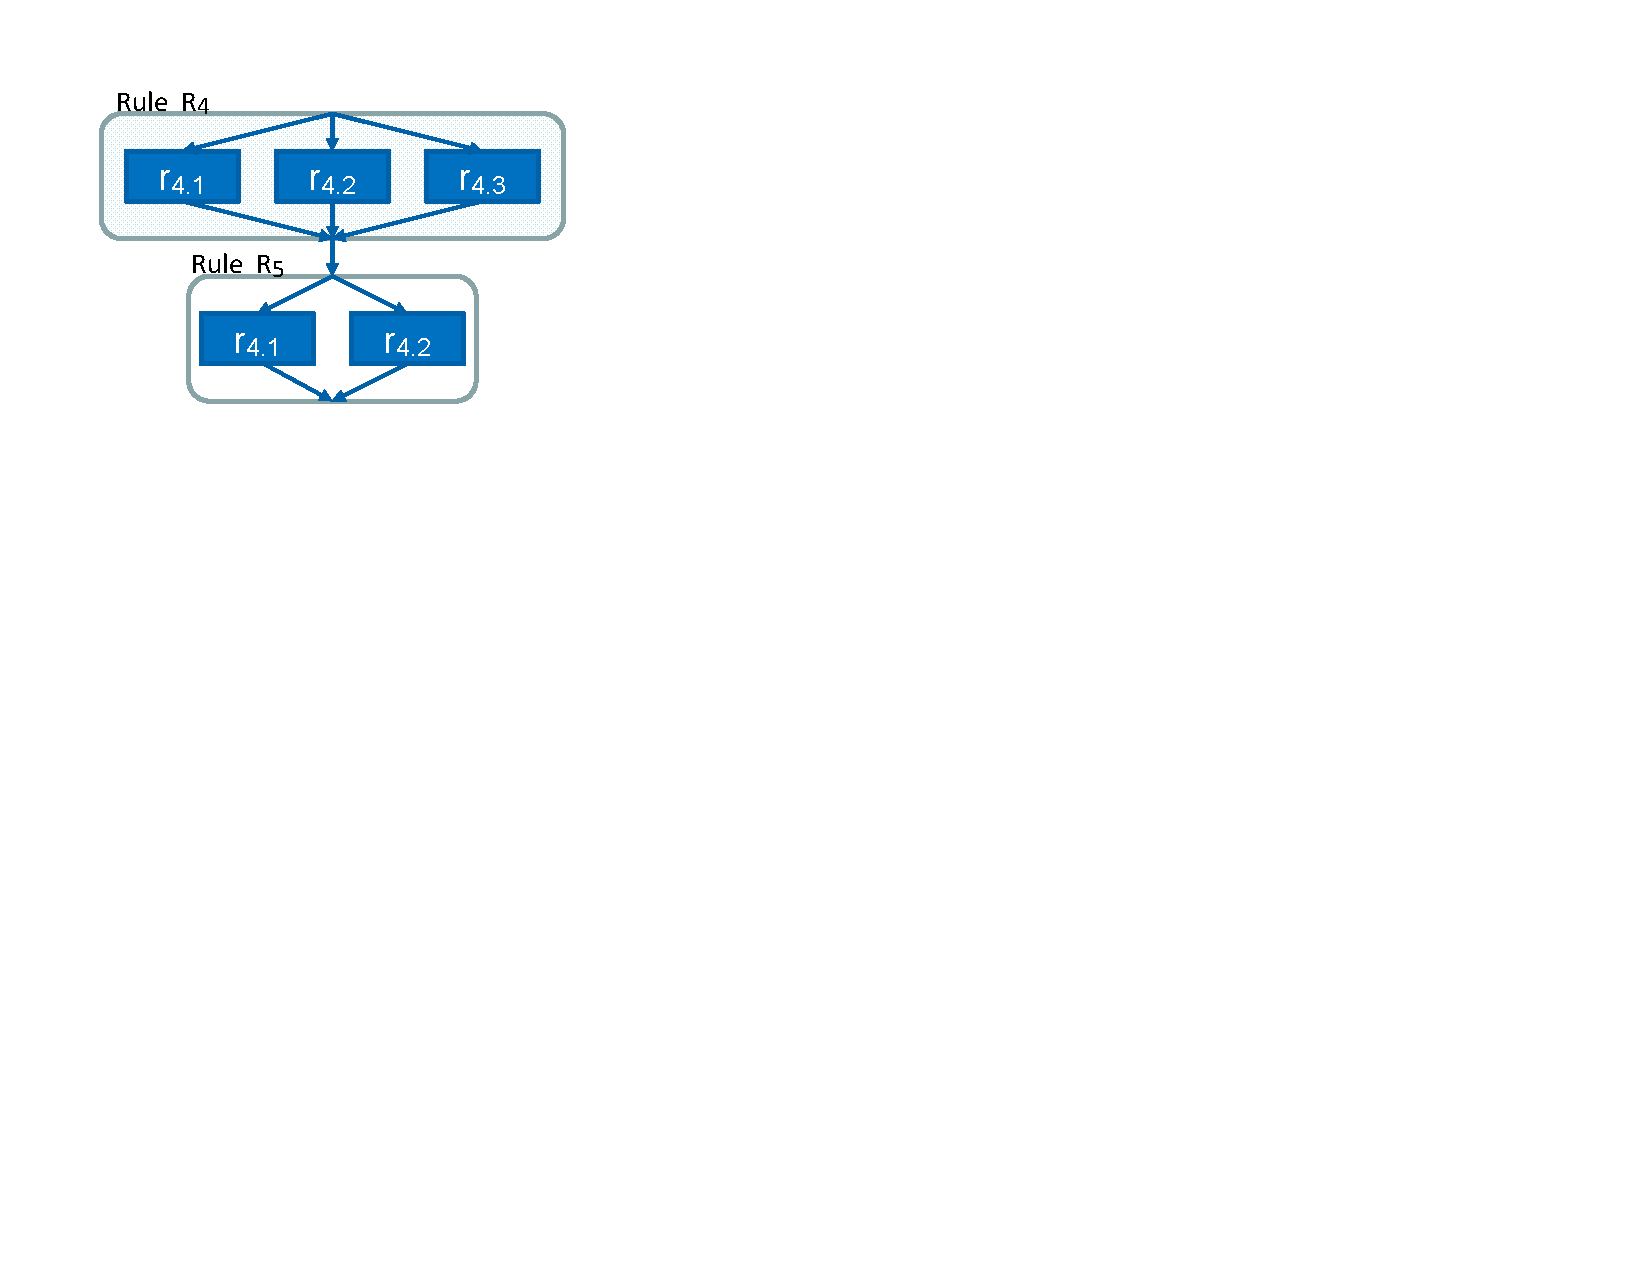
\includegraphics[trim=48 390 520 38,clip,width=2in]{figs/cfg-example.pdf}
\caption{Example operation flow graph for the {\tt Generate Invoice} operation.}
\label{fig:cfg}
\end{figure}

\begin{algorithm}[t]
\footnotesize
\SetAlgoVlined
\KwIn{Operation $op$, RulePart $rp$}
\KwOut{ConcreteSequence $seq$ or $null$}
\BlankLine

\nl Initialize a Queue $queue$ for storing concrete sequences\;
\nl Generate all creation sequences $cseqList$ for the operation $op$\;
\nl \ForEach {creation sequence $cseq \in cseqList$}
{
		\nl Generate all concrete sequences $conSeqList$ for $cseq$\;
		\nl Add all sequences in $conSeqList$ to $queue$\;
} 

\nl \While { queue not empty }
{
		\nl Remove the first concrete sequence $conSeq$ from $queue$\;
		\nl Check whether $conSeq$ is satisfiable\;
		\nl \If {satisfiable}
		{
				\Return $conSeq$ \;
		}
		
		\nl Extract unsatisfiable core $unSatCore$ of $conSeq$\;
		
		/*Ensures that selected operation helps to make progress*/
		\nl \If {$unSatCore$ is already seen}
		{
				Continue\;
		}
		
		\nl Identify operations $opSet$ that help satisfy $unSatCore$\;		
		\nl \ForEach {Operation $candOp$ $\in$ $opSet$}
		{
			\nl Insert $candOp$ to $conSeq$ to generate a list of new concrete sequences $conSeqList$\;
			\nl Add all sequences in $conSeqList$ to $queue$\;			
		}
}

\Return $null$\;
		
\caption{\label{alg:guidedsearch} Algorithm for
  identifying a concrete sequence that cover a given rule part.}
\end{algorithm}



\subsection{Technique}
\label{sec:technique}

We next illustrate our technique using the sample application model shown in Figure~\ref{fig:sample-app}.
Algorithm~\ref{alg:guidedsearch} shows the core algorithm of our technique. We consider
the input operation $op$ as \subject{GenerateInvoice} and the rulepart $rp$ as $RP_{4.2}$.
For brevity,
we omit some details such as exiting the main loop (lines 6-15) when user-defined
threshold on the maximum number of sequences is reached.

\textit{Generate Creation Sequences (Lines 2-5).} Given an operation $op$, our algorithm
first generates creation sequences that produce all entities required for invoking $op$.
Here, a creation sequence is the same as abstract sequence, however, includes only those
operations that create entities and does not include operations that only modify
entities. To generate a creation sequence, our algorithm uses dependency graph of the application.
In particular, it first identifies all input entities of $op$ using the \textit{read}
edges in the graph. For each entity, it identifies operations $cops$ that create those entities
using the \textit{create} edges in the graph. Our algorithm composes sequences by combining
$op$ with operations in $cops$. It next repeats the process if the newly identified
operations require further entities. For our sample application model, the creation sequence for invoking 
the \subject{GenerateInvoice} operation is as follows.

\vspace*{-5pt}
{\small
\begin{alltt}
  State st;
  BalanceType bt;
  Int price;
  Customer cust;
  CreateCustomer(in st,in bt, out cust);
  Order ord;
  CreateOrder(in cust, out ord);	
  Invoice inv;
  GenerateInvoice(in ord, out inv);  
\end{alltt}
}
\vspace*{-5pt}

Note that there can be multiple creation sequences, if the model includes multiple operations
that create the same entity. Next, from each creation sequence,
our algorithm generates concrete sequences by computing all possible combinations of
rule parts among the operations in the sequences. To achieve this, our algorithm
attaches flow graphs of each individual operation in the sequence and then
enumerates all paths in the final flow graph. These concrete sequences generate different
object states for the input entities of the operation $op$. For our current example,
the concrete sequence is as follows. There is only one concrete sequence in our example,
since each of these operations include only one rule part.

\vspace*{-5pt}
{\small
\begin{alltt}
  State st;
  BalanceType bt;
  Int price;
  Customer cust;
  CreateCustomer(in st,in bt, out cust) [\(RP\sb{1.1}\)];
  Order ord;
  CreateOrder(in cust, out ord) [\(RP\sb{3.1}\)];	
  Invoice inv;
  GenerateInvoice(in ord, out inv) [\(RP\sb{4.2}\)];  
\end{alltt}
}
\vspace*{-5pt}

\textit{Check Satisfiability (Line 8).} Next, our algorithm checks whether the 
each concrete sequence in the queue is satisfiable. A concrete sequence 
is considered as satisfiable if it generates desired
object states for all input entities of $op$ that help cover the precondition of the rule
part $rp$. To achieve this, our algorithm constructs a formula composed
of constraints in pre- and post-conditions in each rule part of the sequence. Our algorithm
starts with the precondition of $rp$, referred to as $target$. It next generates
binding constraints that substitute the entities
consumed by the successor operation by the entities created or
modified by the predecessor operation. These binding constraints bind 
the identifiers in the post condition of the predecessor operation to the identifiers of same type
in the pre condition of the successor operation. As the solver has no
notion of objects, the binding must also ensure that object fields
referenced are appropriately bound.

Binding constraints are generated as follows: Assume that we want to
sequence the two operations $O_{pred}$ and $O_{succ}$ and that the
algorithm have chosen rule parts $rp_1$ and $rp_2$ from $O_{pred}$ and
$O_{succ}$, respectively. Now let $v$ be an
identifier of type $\tau$ occurring in either the creates or modifies
clause of $O_{pred}$ and let $w$ be an identifier of the same type
occurring in the input clause of $O_{succ}$. If $\tau$ is an enum type,
the only binding needed is $w = v$. If $\tau$ is an object type, then
we must bind all attributes as well, yielding the following constraint:
$w = v \wedge w.f_1 = v.f_1 \wedge \ldots \wedge w.f_n = v.f_n$ where
$f_1, \ldots , f_n$ are fields declared on $\tau$. If any of the
fields are of object types themselves this process is applied
recursively on each such attribute to generate the final binding
constraint. We repeat this process for all operations in the concrete sequence
and generate final formula. We next pass this formula to a constraint solver to check
whether the formula is satisfiable. If yes, solver also provides values for variables
of enumerated and primitive types, that serve as data passed to each operation
in the sequence.

For the preceding concrete sequence, the solver returns that the composed formula
as unsatisfiable. The reason is that the operation \subject{CreateOrder} sets
the value of attribute \subject{total} in \subject{Order} to zero, whereas the
precondition in rule part $RP_{4.2}$ requires the value of the \subject{total} 
attribute as greater than zero.

\textit{Extract Unsatisfiable Core (Line 10).} If the composed formula is unsatisfiable,
our algorithm extracts the unsatisfiable core of the formula. An unsatisfiable core 
is a subset of the entire formula, which preserves the unsatisfiability but is simplified.
This core helps to suggest additional operations that modify attributes of entities
to produce desired object states. For the current example, our algorithm extracts 
unsatisfied core as 



